\documentclass[11pt,letterpaper,boxed]{hmcpset}
\usepackage{fullpage}
\setlength{\parskip}{6pt}
\setlength{\parindent}{0pt}
\usepackage[margin=1in]{geometry}
\usepackage{graphicx}
\usepackage{enumerate}
\usepackage{marvosym}
\usepackage{amssymb}
\usepackage{wasysym}
\usepackage{gensymb}
\usepackage{mathrsfs}
\usepackage{scrextend}
\usepackage{mathtools}
\usepackage{pgfplots}
\usepackage{xspace}
\usepackage{esvect}
\usepackage{lipsum}
\usepackage{float}
\usepackage{esint}


\name{Name $\rule{4cm}{0.15mm}$}
\class{Physics 51M Section $\rule{.5cm}{0.15mm}$ Box \# $\rule{1cm}{0.15mm}$}
\assignment{Problem Set 9}
\duedate{18 November 2019}

\begin{document}
	
	%\begin{center}
	\noindent\textbf{Collaborators:} 
	%\end{center} 
	
	%\problemlist{}
	
	\begin{problem}  (a) Sketch the vector function $$\Vec{F}(x,y) = -y\hat{x} + x\hat{y}$$ \\
Write down your guess for the direction of the curl of $\vec{F}$ , $\nabla \times \vec{F}$, with a few words of justification.
(b) Calculate the curl of $\vec{F}$ and compare with your prediction in part (a).
(c) Rewrite $\vec{F}$ in cylindrical coordinates, and compute $\nabla \times \vec{F}$ using the cylindrical form of the curl.
Compare with your result from part (b).
		
	\end{problem}
	
	\begin{solution}
		\vfill
	\end{solution}
	\newpage

	\begin{problem} (a) Sketch the following function $\vec{F}(x,y,z)$ in the $z = 1$ plane:
$$\vec{F}(x,y,z) = yz\hat{x} + xz\hat{y} + xy\hat{z}$$ \\
ignoring the out-of-plane $z$-component of $\vec{F}$. Now consider the $z$-component of $\nabla \times \vec{F}$ and write down your guess for its sign.
(b) Calculate the curl of $\vec{F}$ and compare with your prediction in part (a).
	\end{problem}
	\begin{solution}
		\vfill
	\end{solution}
	\newpage
	
	\begin{problem} [Schey: III-15(a)] Verify Stokes's Theorem for $\vec{F} = \vec{i} z^2 - \vec{j} y^2$, $\mathbb{C}$, the square of side 1 lying in the $xz$-plane and directed as shown. Also compute the right-hand side of Stokes's Theorem using surface $S_6$, the square enclosed by the path $\mathbb{C}$ in the $x - z$ plane, and compare with your previous answers.
	\begin{center}
		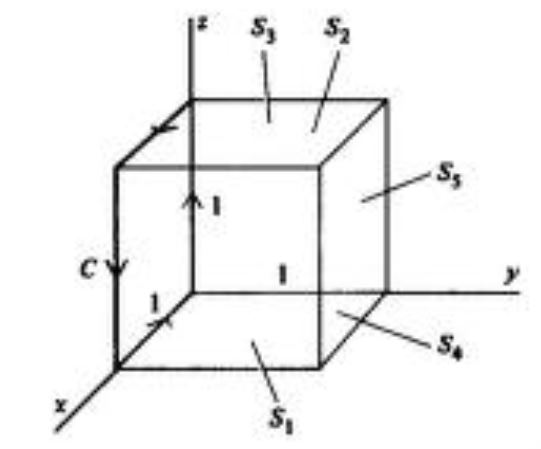
\includegraphics[scale=.5]{51m9pic.jpg}
	\end{center}
	\end{problem}
	\begin{solution}
		\vfill
	\end{solution}
	\newpage
		
	
\end{document}